\thispagestyle{toanhocvadoisongnone}
\pagestyle{toanhocvadoisong}
\everymath{\color{toanhocdoisong}}
\graphicspath{{../toanhocdoisong/pic/}}
\begingroup
\blfootnote{$^1$\color{toanhocdoisong}Hà Nội.}
\AddToShipoutPicture*{\put(0,616){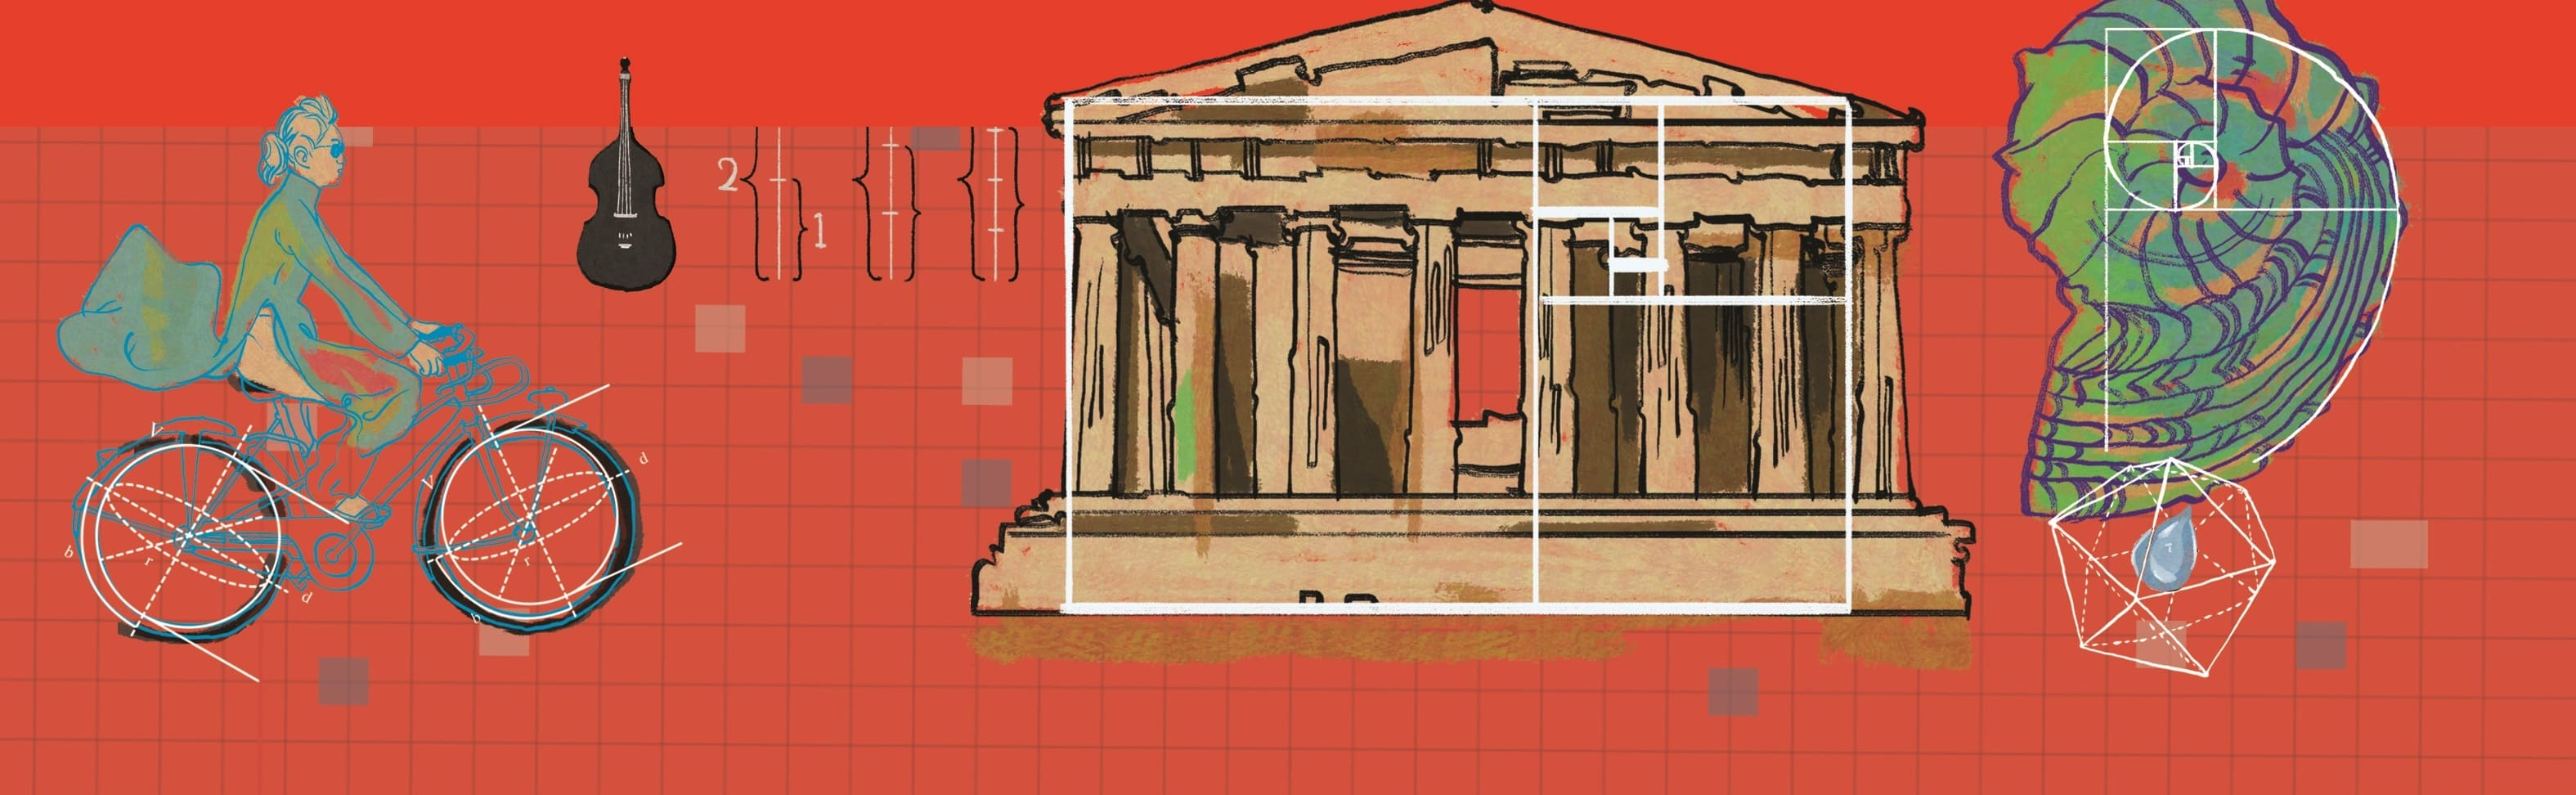
\includegraphics[width=19.3cm]{../bannertoanhocdoisong}}}
\AddToShipoutPicture*{\put(79,520){
\includegraphics[scale=1]{../tieude.pdf}}}
\centering
\endgroup

\vspace*{190pt}

\begin{multicols}{2}
	Bài toán cây kim của Buffon vẫn luôn xuất hiện trong sách giáo khoa toán dưới dạng một phương pháp để tính số $\pi$. Trong bài này, chúng ta hãy cũng Pi tìm hiểu chi tiết về bài toán này cũng như một số ứng dụng thú vị của nó trong thực tiễn.
	\vskip 0.1cm
	\textbf{\color{toanhocdoisong}$\pmb{1.}$ Bài toán cây kim của Buffon}
	\begin{figure}[H]
		\vspace*{-5pt}
		\centering
		\captionsetup{labelformat= empty, justification=centering}
		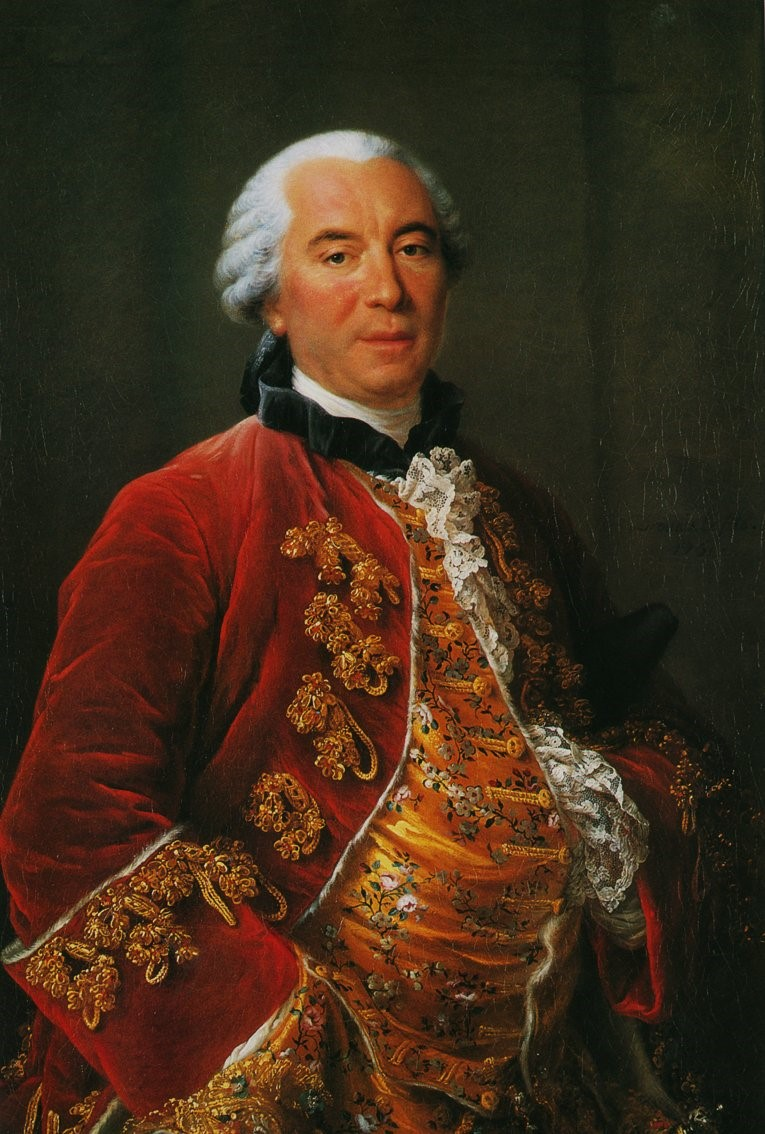
\includegraphics[width=0.6\linewidth]{1}
		\caption{\small\textit{\color{toanhocdoisong}Georges--Louis Leclerc, Comte de Buffon $(1707-1788)$.}}
		\vspace*{-10pt}
	\end{figure}
	Nhà toán học Pháp thế kỉ $18$, Georges Louis Leclerc, được phong Bá tước tại vùng có một ngôi làng tên Buffon nên ông còn có danh hiệu Comte de Buffon (Bá tước Buffon). Do đó các tài liệu thường gọi tắt là Buffon. Bài toán nổi tiếng mang tên ông có nội dung như sau:
	\vskip 0.1cm
	``Trên một tờ giấy với các đường kẻ cách đều nhau khoảng cách $d$, thả ngẫu nhiên một cây kim chiều dài $l$ $(d>l)$, hãy tìm xác suất để cây kim cắt một đường nằm ngang trên trang giấy".
	\begin{figure}[H]
		\vspace*{-5pt}
		\centering
		\captionsetup{labelformat= empty, justification=centering}
		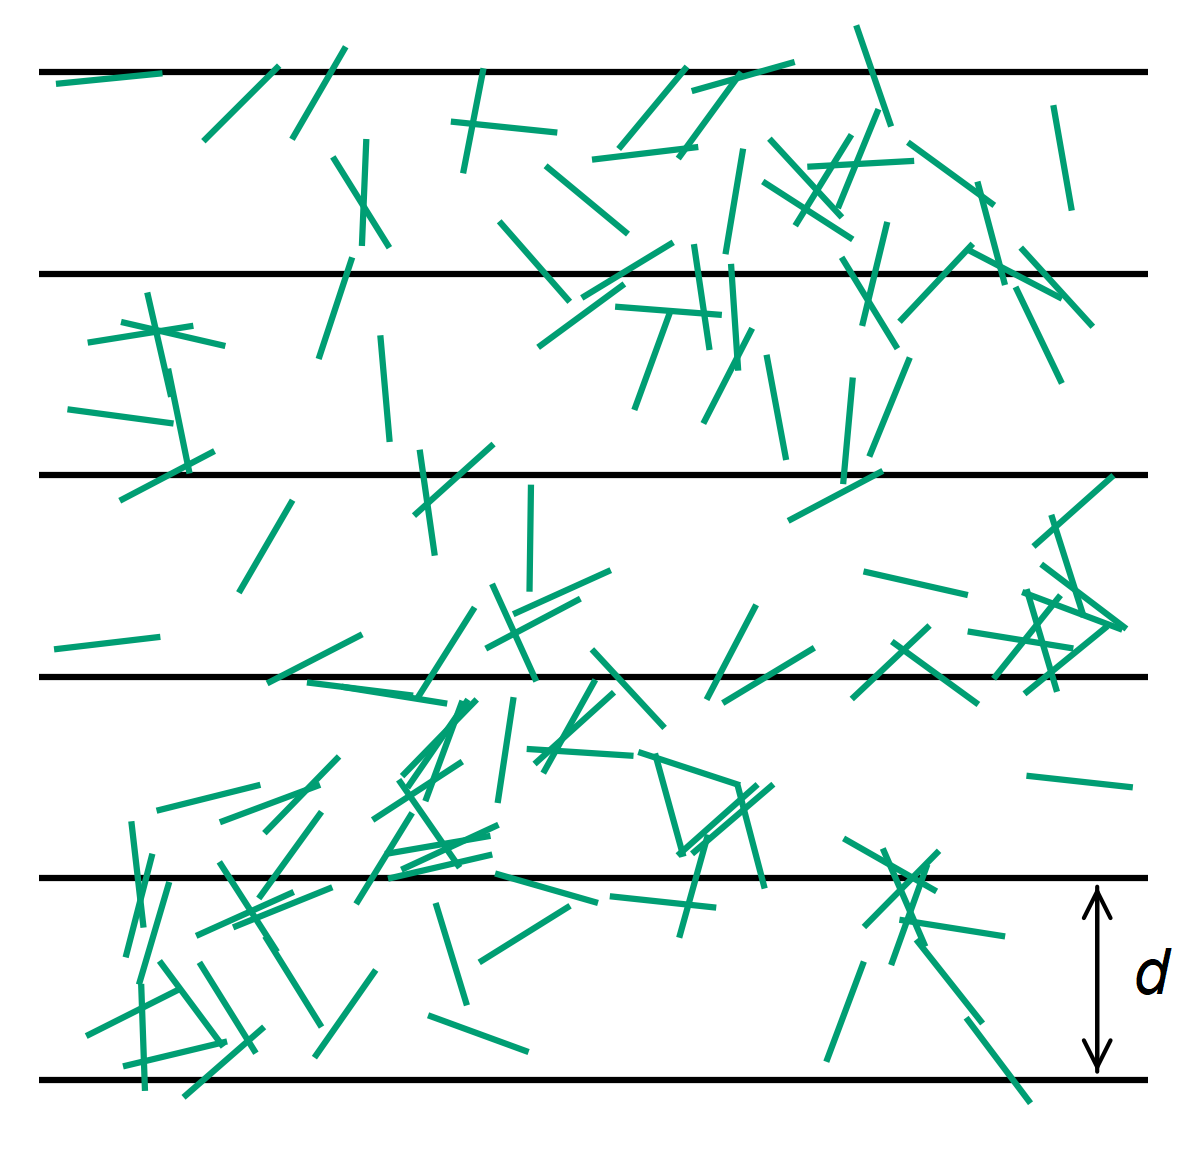
\includegraphics[width=0.95\linewidth]{2}
		\caption{\small\textit{\color{toanhocdoisong}Hình $1$. Minh họa bài toán cây kim của Buffon.}}
		\vspace*{-10pt}
	\end{figure}
	Chúng ta hãy xét một lời giải không sử dụng tích phân được E. Barbier đưa ra năm $1860$.
	\vskip 0.1cm 
	Do $l<d$ nên chỉ có hai trường hợp xảy ra: cây kim cắt một đường kẻ và cây kim không đè lên đường kẻ nào; không tồn tại trường hợp cây kim cắt nhiều hơn một đường kẻ.
	\vskip 0.1cm
	Gọi $P(l)$ là xác suất để cây kim có độ dài $l$ cắt một đường kẻ khi được thả. Lấy một điểm bất kỳ trên cây kim chia nó thành hai đoạn thẳng độ dài $l_1$ và $l_2$. Ta có:
	\begin{align*}
		P(l)=P(l_1 )+P(l_2).
	\end{align*}
	Quan hệ trên có thể được mở rộng ra thành dạng $P(l)=n\cdot P(\dfrac{l}{n})$. Tức là xác suất để một cây kim cắt đường kẻ khi được thả sẽ bằng $n$ lần xác suất này của cây kim có độ dài bằng $\dfrac{1}{n}$ lần độ dài cây kim ban đầu.
	\vskip 0.1cm
	Do đó, $P(l)=c\cdot l$ với $c$ là một hằng số, $c=P(1)$ (khi $l=1$ và $d > 1$).
	\begin{figure}[H]
		\vspace*{-5pt}
		\centering
		\captionsetup{labelformat= empty, justification=centering}
		\begin{tikzpicture}[scale=0.58]
			\definecolor{qqqqff}{rgb}{0.,0.,1.}
			\definecolor{ududff}{rgb}{0.30196078431372547,0.30196078431372547,1.}
				\fill[line width=0.8pt,color=cackithi,fill=cackithi,fill opacity=0.5] (1.,3.) -- (3.,5.) -- (2.267949192431123,7.732050807568878) -- (-0.46410161513775494,8.464101615137755) -- (-2.4641016151377553,6.464101615137756) -- (-1.7320508075688794,3.7320508075688785) -- cycle;
				\draw [line width=0.8pt,color=toanhocdoisong] (1.,3.)-- (3.,5.);
				\draw [line width=0.8pt,color=toanhocdoisong] (3.,5.)-- (2.267949192431123,7.732050807568878);
				\draw [line width=0.8pt,color=toanhocdoisong] (2.267949192431123,7.732050807568878)-- (-0.46410161513775494,8.464101615137755);
				\draw [line width=0.8pt,color=toanhocdoisong] (-0.46410161513775494,8.464101615137755)-- (-2.4641016151377553,6.464101615137756);
				\draw [line width=0.8pt,color=toanhocdoisong] (-2.4641016151377553,6.464101615137756)-- (-1.7320508075688794,3.7320508075688785);
				\draw [line width=0.8pt,color=toanhocdoisong] (-1.7320508075688794,3.7320508075688785)-- (1.,3.);
				\draw [toanhocdoisong,line width=0.8pt] (-6.,6.)-- (6.,6.);
				\draw [toanhocdoisong,line width=0.8pt] (-6.,2.)-- (6.,2.);
				\draw [toanhocdoisong,line width=0.8pt] (-6.,10.)-- (6.,10.);
			
				\draw [fill=cackithi] (1.,3.) circle (2.5pt);
				\draw [fill=cackithi] (3.,5.) circle (2.5pt);
				\draw [fill=cackithi] (2.267949192431123,7.732050807568878) circle (2.5pt);
				\draw [fill=cackithi] (-0.46410161513775494,8.464101615137755) circle (2.5pt);
				\draw [fill=cackithi] (-2.4641016151377553,6.464101615137756) circle (2.5pt);
				\draw [fill=cackithi] (-1.7320508075688794,3.7320508075688785) circle (2.5pt);
		\end{tikzpicture}
		\caption{\small\textit{\color{toanhocdoisong}Hình $2$. Thả một đa giác cạnh $l$ lên tờ giấy với các đường kẻ ngang cách đều nhau.}}
		\vspace*{-10pt}
	\end{figure}
	Ta hãy tiếp tục xét một đa giác đều $N$ cạnh có độ dài mỗi cạnh bằng $l$ (Hình $2$). Ta đã biết ở trên rằng xác suất để mỗi cạnh của đa giác cắt một đường kẻ là $P(l)$. Đây cũng chính là giá trị kỳ vọng của số giao điểm của một cạnh với các đường kẻ, vì số giao điểm nói chung chỉ có thể là $0$ hoặc $1$ tương ứng với không cắt và cắt. Theo tính chất cộng tính của kỳ vọng, giá trị kỳ vọng của số giao điểm của đa giác với các đường kẻ khi thả lên tờ giấy là:
	\begin{align*}
		E &= \sum\nolimits_{i = 1}^N {P(l) = N \cdot } P(l) \\
		&= N \cdot c \cdot l = c \cdot L, \tag{$1$}
	\end{align*}
	với $L=N \cdot l$ là chu vi của đa giác đều.
	\vskip 0.1cm
	\columnbreak
	\PIbox{\textbf{\color{toanhocdoisong}Giá trị kỳ vọng}
		\vskip 0.1cm
		Trong một thí nghiệm ngẫu nhiên, nếu kết quả có giá trị $x_i$ có xác suất xảy ra là $p_i$ thì giá trị kỳ vọng của kết quả thu được được tính theo công thức:
		\setlength{\abovedisplayskip}{4pt}
		\setlength{\belowdisplayskip}{4pt}
		\begin{align*}
			E=x_1 p_1+x_2 p_2+ \cdots +x_n p_n.
		\end{align*}
		Ví dụ, với thí nghiệm gieo con xúc xắc, giá trị kỳ vọng của số chấm thu được là:
		\begin{align*}
			E=\frac{1}{6}\cdot 1 + \frac{1}{6} \cdot 2 + \cdots + \frac{1}{6}\cdot6 = 3{,5}.
		\end{align*}
		Chú ý rằng giá trị kỳ vọng có thể không trùng với một trong các giá trị có thể xảy ra. Theo định luật số lớn trong xác suất, với số lần thực hiện thí nghiệm càng lớn thì giá trị trung bình của các kết quả sẽ càng đến gần với giá trị kỳ vọng.}
	\vskip 0.1cm
	Mặt khác, nếu giữ chu vi $L$ của đa giác không đổi, khi $N \to \infty$, đa giác của ta sẽ trở thành một đường tròn có chu vi $L$ và bán kính $\dfrac{L}{2\pi}$.
	\vskip 0.1cm
	Để tính hệ số $c$, ta xét một trường hợp đặc biệt, khi đường tròn có đường kính đúng bằng khoảng cách $d$ giữa các dòng kẻ. Khi đó, ta có $L=\pi d$.
	\begin{figure}[H]
		\vspace*{-5pt}
		\centering
		\captionsetup{labelformat= empty, justification=centering}
		\begin{tikzpicture}[scale=0.58]
			\draw [toanhocdoisong, line width=1.pt] (-6.,6.)-- (6.,6.);
			\draw [toanhocdoisong, line width=1.pt] (-6.,10.)-- (6.,10.);
			\draw [cackithi, line width=1.pt] (2.8,8.) circle (1.97cm);
			\draw [cackithi, line width=1.pt] (-2.8,6.) circle (1.97cm);
		\end{tikzpicture}
		\caption{\small\textit{\color{toanhocdoisong}Hình $3$. Đường tròn có đường kính $d$ sẽ luôn cắt một đường kẻ tại hai điểm hoặc tiếp xúc hai đường kẻ.}}
		\vspace*{-10pt}
	\end{figure}
	Đường tròn có đường kính $d$ sẽ luôn cắt một đường kẻ tại $2$ giao điểm hoặc tiếp xúc với $2$ đường kẻ liên tiếp, do đó với đường tròn này $E=2$. Thay vào ($1$) ta có:
	\begin{align*}
		2=c\cdot\pi d
	\end{align*}
	hay $c = \dfrac{2}{\pi d}$.
	\vskip 0.1cm
	Vậy xác suất để một cây kim khi thả cắt đường nằm ngang trên giấy là 
	\begin{align*}
		P(l) = \frac{2l}{\pi d}. \tag{$2$}
	\end{align*}
	\begin{figure}[H]
		\vspace*{-5pt}
		\centering
		\captionsetup{labelformat= empty, justification=centering}
		\begin{tikzpicture}[scale=0.58]
			\draw [shift={(-1.,8.)},line width=0.8pt,color=cackithi,fill=cackithi,fill opacity=0.15000000596046448] (0,0) -- (0.:0.7555063451882832) arc (0.:26.56505117707799:0.7555063451882832) -- cycle;
			\draw [toanhocdoisong,line width=0.8pt] (-6.,10.)-- (6.,10.);
			\draw [toanhocdoisong,dashed, line width=0.8pt] (-6.,9.)-- (6.,9.);
			\draw [toanhocdoisong,dashed, line width=0.8pt] (-6.,8.)-- (6.,8.);
			\draw [toanhocdoisong,dashed, line width=0.8pt] (-6.,7.)-- (6.,7.);
			\draw [toanhocdoisong, line width=0.8pt] (-6.,5.)-- (6.,5.);
			\draw [cackithi,line width=0.8pt] (-3.,7.)-- (1.,9.);
			\draw [fill=cackithi] (-3,7) circle (2.5pt);
			\draw [fill=cackithi] (1,9) circle (2.5pt);
			\draw [fill=cackithi] (-1,8) circle (2.5pt);
			\draw [cackithi,-stealth,line width=0.8pt] (3.,8.)-- (3.,9.);
			\draw [cackithi,-stealth,line width=0.8pt] (3.,8.)-- (3.,7.);
			
			\draw[color=cackithi] (0.65,8.347966297286694) node {$\color{cackithi}\alpha$};
			\draw[color=cackithi] (4.2,8.5) node {$\color{cackithi}l\sin\alpha$};
		\end{tikzpicture}
		\caption{\small\textit{\color{toanhocdoisong}Hình $4$. Chứng minh công thức $(2)$ sử dụng tích phân.}}
		\vspace*{-10pt}
	\end{figure}
	Ta cũng có thể thu được đáp án này bằng cách sử dụng tích phân. Cụ thể là ta xây dựng một mô hình xác suất cho vị trí rơi của cây kim. Gọi $\alpha$ $(0\le \alpha \le \dfrac{\pi}{2})$ là góc mà cây kim tạo với phương nằm ngang. Hình chiếu của nó theo phương vuông góc với các đường kẻ sẽ có độ dài $l\sin\alpha$, mà khoảng cách giữa hai đường kẻ là $d$, do đó xác suất để nó cắt một đường kẻ là $\dfrac{l\sin\alpha}{d}$. Coi phân bố của $\alpha$ là đều trên khoảng $[0,\dfrac{\pi}{2}]$, ta tính giá trị trung bình bằng cách lấy tích phân trên khoảng này rồi chia cho $\dfrac{\pi}{2}$ để thu được ($2$):
	\begin{align*}
		P(l) &= \frac{2}{\pi }\int_0^{\frac{\pi }{2}} {\frac{{l\sin \alpha }}{d}} d\alpha  = \frac{2}{\pi }\frac{l}{d}\left[ { - \cos \alpha } \right]|_0^{\frac{\pi }{2}}\\
		& = \frac{2}{\pi }\frac{l}{d}.
	\end{align*}
	Với cây kim có độ dài lớn hơn $d$, xác suất để nó cắt ít nhất một đường kẻ trong khoảng $\left[\arcsin\left(\dfrac{d}{l}, \dfrac{\pi}{2}\right)\right]$ sẽ luôn là $1$, do đó:
	\begin{align*}
		&P(l) \\
		= \,&\frac{2}{\pi }\left( {\int_0^{\arcsin \left( {\frac{d}{l}} \right)} {\frac{{l\sin \alpha }}{d} + } \int_{\arcsin \left( {\frac{d}{l}} \right)}^{\frac{\pi }{2}} {1d\alpha } } \right)\\
		=\,&1 \!\!+\!\! \frac{2}{\pi }\!\left( \!\!{\frac{l}{d}\!\!\left(\!\! {1 \!-\! \sqrt {\!\!1 \!-\! \frac{{{d^2}}}{{{l^2}}}} \!} \right) \!\!-\! \arcsin\! \frac{d}{l}}\! \right)\!\!.\tag{$3$}
	\end{align*}
	Bài toán này cũng được Laplace mở rộng cho trường hợp lưới trên tờ giấy là lưới chữ nhật và  tính xác suất để cây kim không cắt một đường kẻ dọc hay ngang nào. 
	\vskip 0.1cm
	Cũng chính Laplace đã đề xuất sử dụng thí nghiệm này để tính giá trị của số $\pi$. Đây cũng là khía cạnh được biết đến nhiều nhất về bài toán cây kim của Buffon. Thật vậy, nếu trong $M$ lần thả cây kim, ta thu được $m$ lần mà nó cắt một đường kẻ, công thức ($2$) cho ta:
	\begin{align*}
		\pi = \frac{2l}{d\cdot\left(\frac{m}{M}\right)},
	\end{align*}
	với $\dfrac{m}{M}$ là xác suất thực nghiệm của sự kiện cây kim cắt một đường kẻ.
	\vskip 0.1cm
	Đề xuất này của Laplace rất gần với phương pháp Monte Carlo của hơn một thế kỉ sau. Tuy vậy, về mặt thực tế, nó gập phải một số vấn đề. Nhiều thí nghiệm được tiến hành và cho kết quả của $\pi$ không quá chính xác: $3{,}1596$; $3{,}1553$; $3{,}137$.
	\vskip 0.1cm 
	Năm $1901$, Lazzarini công bố giá trị $3{,}1415929$ cho $3408$ lần thả cây kim, một giá trị khá chính xác (so với giá trị đã biết hiện nay, thì chỉ có chữ số cuối là không đúng). Tuy vậy, một số nghiên cứu đã chỉ ra kết quả này hầu như là ngụy tạo. Theo các lí thuyết về ước lượng tham số, để có độ chính xác đến $6$ chữ số sau dấu phẩy, cần phải tiến hành thí nghiệm trên $1{,}34×10^{14}$ lần chứ không phải vài nghìn lần. Đồng thời, số liệu của Lazzarini sử dụng phân số $\dfrac{355}{113}$, một số hữu tỉ được biết là một xấp xỉ tốt cho $\pi$. 
	\vskip 0.1cm
	Ngay cả với máy tính điện tử thì việc ước lượng $\pi$ bằng cách sử dụng thí nghiệm Buffon cũng không đạt được độ chính xác quá cao do việc làm tròn số trên máy tính. Đồng thời, các chữ số của $\pi$ cũng có thể được tính toán một cách chính xác hơn bởi các phương pháp khác.
	\vskip 0.1cm
	Tuy vậy, bài toán cây kim của Buffon có một ý nghĩa quan trọng trong lịch sử toán học bởi sự liên hệ giữa xác suất và hình học. Đây là một hướng tiếp cận mới khác với hướng tiếp cận xác suất sử dụng tổ hợp như truyền thống.
	\vskip 0.1cm
	\textbf{\color{toanhocdoisong}Bài tập}
	\vskip 0.1cm
	$1$. Chứng minh rằng khi cây kim vô cùng dài thì một cách hầu chắc chắn nó sẽ luôn cắt ít nhất một đường kẻ, tức là biểu thức trong ($3$) có giới hạn là $1$ khi $l\to \infty$.
	\vskip 0.1cm
	$2$. Trên tờ giấy với các đường kẻ ngang cách nhau khoảng $d$, thả ngẫu nhiên một đường tròn với bán kính $r < \dfrac{d}{2}$. Hãy tính xác suất để đường tròn cắt và không cắt các đường kẻ.
	\vskip 0.1cm
	$3$. Tương tự bài trên nhưng thả một hình vuông có cạnh $a<d$. Hãy tính xác suất để số giao điểm của các cạnh hình vuông với các đường kẻ ngang là:
	\vskip 0.1cm
	$a)$ $0$\quad\quad		$b)$ $1$\quad\quad		$c)$ $2$\quad\quad
	$d)$ $3$\quad\quad		$e)$ $4$
	\vskip 0.1cm
	Gợi ý: Xét trường hợp $a<\dfrac{d}{\sqrt{2}}$ và $a> \dfrac{d}{\sqrt{2}}$.
	\vskip 0.1cm	
	$4$. Trong thí nghiệm Buffon, với cây kim có độ dài $l>d$, hãy chứng minh giá trị kỳ vọng của số giao điểm của cây kim với các đường kẻ ngang là $E = \dfrac{2l}{\pi d}$. (Gợi ý: Gọi $N$ là số nguyên lớn nhất sao cho $d<\dfrac{l}{N}$, coi cây kim là hình gồm $N$ đoạn thẳng bằng nhau).
	\vskip 0.1cm
	$5$. Mở rộng của Laplace. Trên một lưới chữ nhật, với mỗi hình chữ nhật có chiều dài $a$ và chiều rộng $b$, thả ngẫu nhiên một cây kim chiều dài $l$ (biết rằng $l$ nhỏ hơn cả $a$ và $b$). Hãy tính xác suất để cây kim không chạm bất kỳ cạnh nào của lưới.
	\vskip 0.1cm
	$6$. Lưới Uspensky. Cho một lưới tam giác đều như hình vẽ với $d$ là chiều cao của mỗi tam giác đều. Thả một cây kim chiều dài \linebreak$l<d$ lên lưới tam giác đều này. Hãy tính xác suất để số giao điểm của cây kim với các đường trong lưới là:
	\vskip 0.1cm
	\quad\quad$a)$ $0$\quad\quad		$b)$ $1$\quad\quad		$c)$ $2$	\quad\quad	$d)$ $3$
	\begin{figure}[H]
		\vspace*{5pt}
		\centering
		\captionsetup{labelformat= empty, justification=centering}
		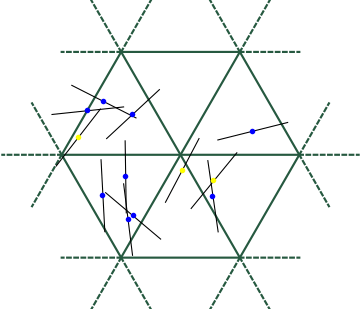
\includegraphics[width=1\linewidth]{6}
		\vspace*{-15pt}
	\end{figure}
	$7$. Bài toán sợi mì của Buffon. Trên một tờ giấy với các đường kẻ ngang song song cách nhau khoảng $d$, ném ngẫu nhiên một sợi mì ướt có độ dài $l$. Chứng minh rằng giá trị kì vọng của số giao điểm của sợi mì với các đường kẻ ngang là $E=\dfrac{2l}{\pi d}$. Giả sử rằng khi ném sợi mì, chiều dài của nó không đổi nhưng nó có thể uốn thành một đường cong bất kỳ.
	\vskip 0.1cm
	\textbf{\color{toanhocdoisong}$\pmb{2.}$ Đo độ dài bằng phương pháp ngẫu nhiên}
	\vskip 0.1cm
	Với một số thay đổi, thí nghiệm của Buffon có thể được sử dụng để giải quyết một vấn đề thực tế trong khoa học: đo độ dài của rễ cây (Newman, $1966$). Xét một bản thủy tinh mà trên đó một mẫu vật (ví dụ rễ cây) được trải phẳng. Khi quan sát mẫu vật qua kính hiển vi, người ta sử dụng một thị kính với một đường sợi tóc để soi các vùng khác nhau của bản thủy tinh.
	\vskip 0.1cm
	Với mỗi lần quan sát, thị kính được quay một góc bất kì và đường sợi tóc cũng được quay theo. Sau đó, số giao điểm của đường sợi tóc với rễ cây sẽ được ghi lại. Cách thức này được lặp lại nhiều lần với các vị trí quan sát ngẫu nhiên khác nhau trên bản thủy tinh. Để tiện lợi hơn, ta có thể đặt bản thủy tinh trên một tấm giấy với các điểm ngẫu nhiên đã được đánh dấu trước. Các điểm quan sát cũng có thể là một lưới ô vuông các điểm cách đều.
	\begin{figure}[H]
%		\vspace*{5pt}
		\centering
		\captionsetup{labelformat= empty, justification=centering}
		
\includegraphics[width=1\linewidth]{7}
		
\includegraphics[width=1\linewidth]{8}
		\caption{\small\textit{\color{toanhocdoisong}Hình $5$. Trên: Thị kính của kính hiển vi có đường sợi tóc (đường thẳng đứng). Dưới: minh họa phép đo độ dài rễ cây (màu xanh) với các vị trí và góc quay khác nhau của đường sợi tóc (màu đỏ). Số lượng đường sợi tóc trong hình chỉ mang tính minh họa, trong thực tế, cấu trúc rễ cây càng phức tạp thì số lượng đường sợi tóc cần sử dụng lại càng nhiều. Mỗi lần quan sát qua kính, ta chỉ thấy được một vùng hình tròn có đường kính là đường sợi tóc.}}
		\vspace*{-10pt}
	\end{figure}
	Về mặt bản chất, thay vì đếm số giao điểm của cây kim được thả ngẫu nhiên với các đường kẻ ngang, ta đếm số giao điểm của các đường sợi tóc được phân bố ngẫu nhiên với mẫu vật rễ cây (gồm nhiều đường cong) trên bản thủy tinh.
	\vskip 0.1cm
	Độ dài của rễ cây có thể được tính theo công thức:
	\begin{align*}
		R= \frac{\pi N A}{2H},	\tag{$4$}
	\end{align*}
	với $N$ là số giao điểm đã được đếm, $A$ là diện tích bản thủy tinh và $H$ là tổng độ dài của tất cả các đường sợi tóc.
	\vskip 0.1cm
	Thật vậy, xét một đoạn rễ cây $PQ$ có chiều dài $\Delta R$ và một đường sợi tóc $MN$ chiều dài $h$. Nếu khoảng cách từ trung điểm $D$ của $PQ$ đến $MN$ lớn hơn $\dfrac{1}{2}\Delta R$ thì $PQ$ và $MN$ chắc chắn không cắt nhau. Miền giới hạn này được biểu diễn bằng đường nét đứt trong hình. Giả sử $\dfrac{\Delta R}{h}$ là nhỏ, diện tích miền này có thể được xấp xỉ bằng $\Delta R \cdot h$. Do $MN$ được phân bố ngẫu nhiên trên bản thủy tinh, xác suất để $D$ nằm trong miền này là $\dfrac{\Delta R \cdot h}{A}$.
	\vskip 0.1cm
	Khi $D$ nằm trong miền cách $MN$ một khoảng không quá $\dfrac{1}{2}\Delta R$, khoảng cách từ $D$ đến $MN$ cần phải không lớn hơn $\dfrac{1}{2}\Delta R |\sin \theta |$, với $\theta$ là góc tạo bởi hai đường thẳng $PQ$ và $MN$, để $PQ$ và $MN$ cắt nhau. Xác suất để $PQ$ và $MN$ cắt nhau khi $D$ đã nằm trong miền trên là:
	\begin{align*}
		\frac{\frac{1}{2}\Delta R|\sin\theta|}{\frac{1}{2}\Delta R} = |\sin\theta|.
	\end{align*}
	Do đó, theo công thức nhân xác suất, xác suất để $PQ$ và $MN$ cắt nhau là:
	\begin{align*}
		p = \frac{\Delta R\cdot h}{A} |\sin\theta|.
	\end{align*}
	\begin{figure}[H]
		\vspace*{-5pt}
		\centering
		\captionsetup{labelformat= empty, justification=centering}
		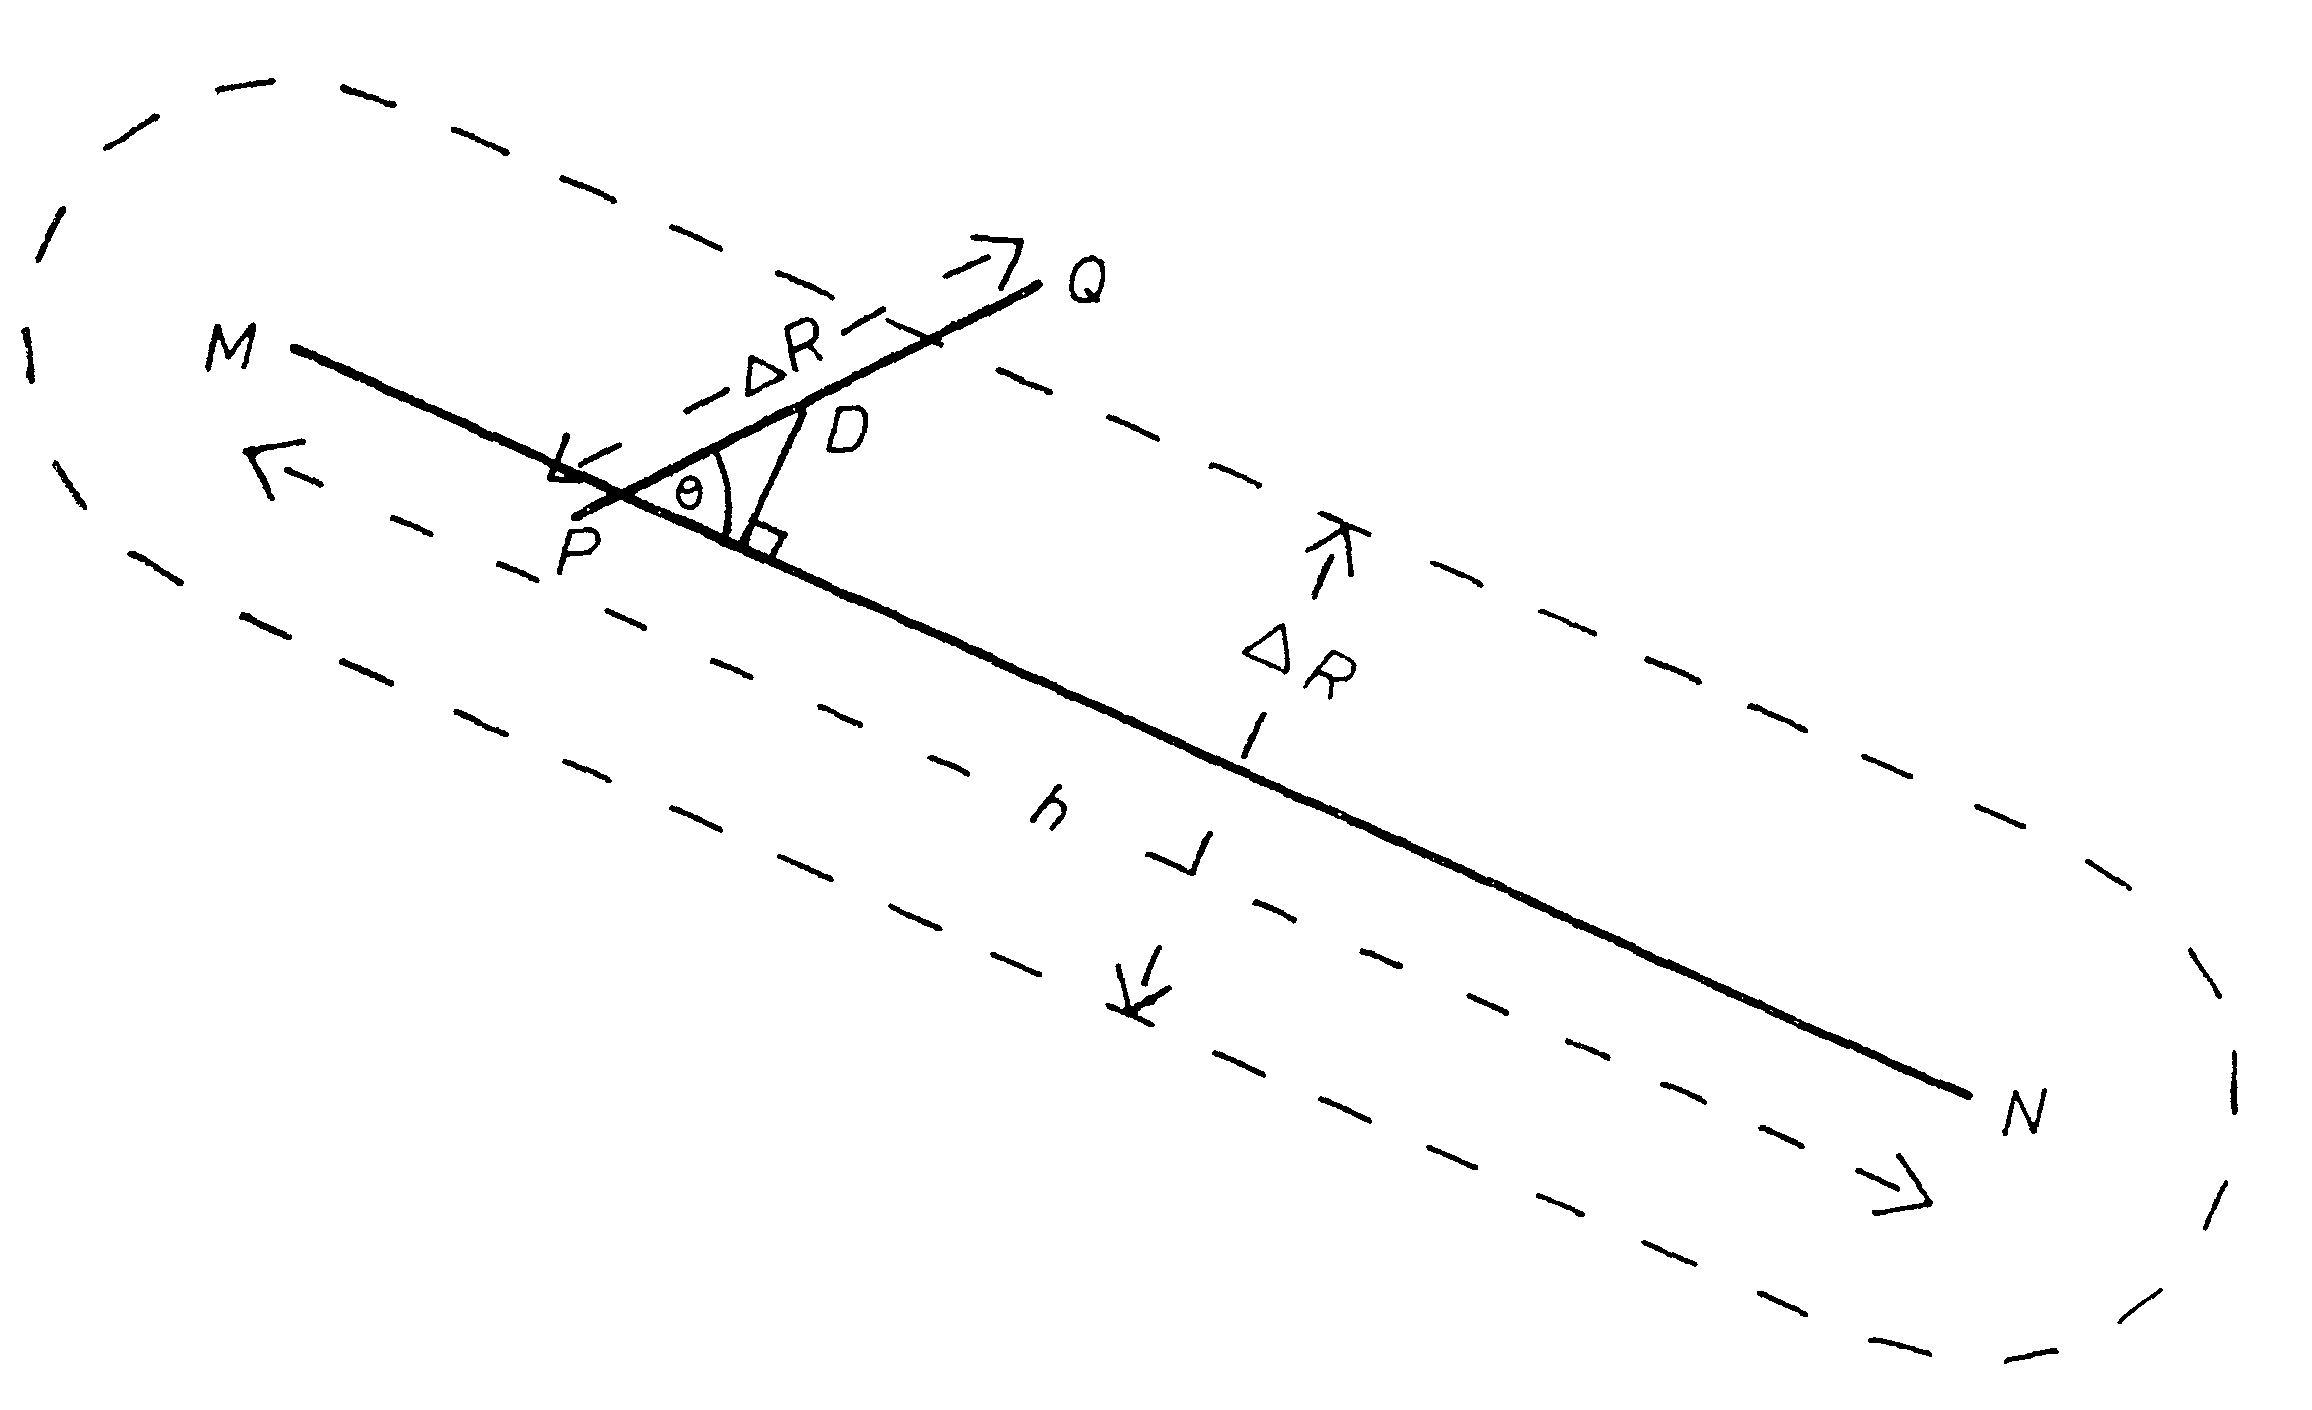
\includegraphics[width=1\linewidth]{9}
		\caption{\small\textit{\color{toanhocdoisong}Hình $6$. Đoạn rễ cây $PQ$ và đường sợi tóc $MN$.}}
		\vspace*{-10pt}
	\end{figure}
	Tổng độ dài của các đoạn sợi tóc được phân bố ngẫu nhiên trên miền diện tích $A$ là $H$. Các góc $\theta$ cũng nhận giá trị ngẫu nhiên trong khoảng $[0,2\pi]$ nên giá trị kì vọng của số giao điểm của $PQ$ với các đường sợi tóc là:
	\begin{align*}
		\frac{1}{2\pi}\int_0^{2\pi}{\frac{{\Delta R \cdot H}}{A}}|\sin\theta|d\theta= \frac{2\left(\Delta R \cdot H\right)}{\pi A}.
	\end{align*}
	Coi rễ cây là một hình với nhiều đoạn có độ dài $\Delta R$, ta được giá trị kì vọng của số giao điểm của rễ cây với tất cả các đường sợi tóc là:
	\begin{align*}
		N = \frac{2RH}{\pi A}.
	\end{align*}
	Do $N$ là giá trị kỳ vọng nên khi đo đạc người ta cần phải tiến hành nhiều lần quan sát với các vị trí ngẫu nhiên của đường sợi tóc để kết quả thí nghiệm gần với giá trị của $N$ trong công thức.
	\vskip 0.1cm
	Ví dụ, với bản thủy tinh $10\times 20$ cm; tiến hành quan sát $40$ lần, độ dài đường sợi tóc (đường kính của thị trường vùng quan sát được) là $1{,}88$ cm; số giao điểm quan sát được là $344$ thì tổng độ dài của rễ cây là:
	\begin{align*}
		R - \frac{\pi \cdot 344\cdot 10 \cdot 20}{2\cdot40 \cdot1{,}88} = 1436 \text{ cm}.
	\end{align*}
	Cách đo độ dài này đã được các nhà thực vật học sử dụng trong nhiều thập kỉ mãi cho đến gần đây mới được thay thế bởi các phần mềm xử lí ảnh từ các camera có độ phân giải cao.
	\vskip 0.1cm
	\textbf{\color{toanhocdoisong}$\pmb{3.}$ Kiến biết đo diện tích bằng xác suất?}
	\vskip 0.1cm
	Phương pháp đo độ dài ở phần trước cũng có thể được biến đổi để tiến hành đo diện tích.
	\vskip 0.1cm
	Một nghiên cứu khá thú vị trên loài kiến \textit{Leptothorax albipennis} đưa ra giả thuyết rằng loài kiến này đã sử dụng xác suất để tính diện tích khi chọn tổ (kiến thường cố gắng chọn tổ có diện tích lớn nhất trong các vị trí khảo sát) (Mallon \& Franks, $2000$).
	\vskip 0.1cm
	Khi sử dụng camera để theo dõi kiến trinh sát trong phòng thí nghiệm, người ta thấy trong lần thứ nhất đến một vị trí để khảo sát, con kiến sẽ đi một cách ngẫu nhiên trong hộp theo một đường cong bao phủ phần lớn các vị trí trong hộp (gọi là đường cong $L$). Trong những lần tiếp theo (thường nó sẽ quay lại lần thứ hai hoặc có thể là lần thứ $3$), nó sẽ đi một đường cong đơn giản hơn (gọi là đường cong $S$). Đồng thời, khi đến các vị trí đã đi qua (kiến khi di chuyển có thể tiết ra pheromone để đánh dấu đường đi của mình), tức là các giao điểm của $L$ và $S$, kiến dành thời gian lâu hơn nhiều.
	\begin{figure}[H]
		\vspace*{-5pt}
		\centering
		\captionsetup{labelformat= empty, justification=centering}
		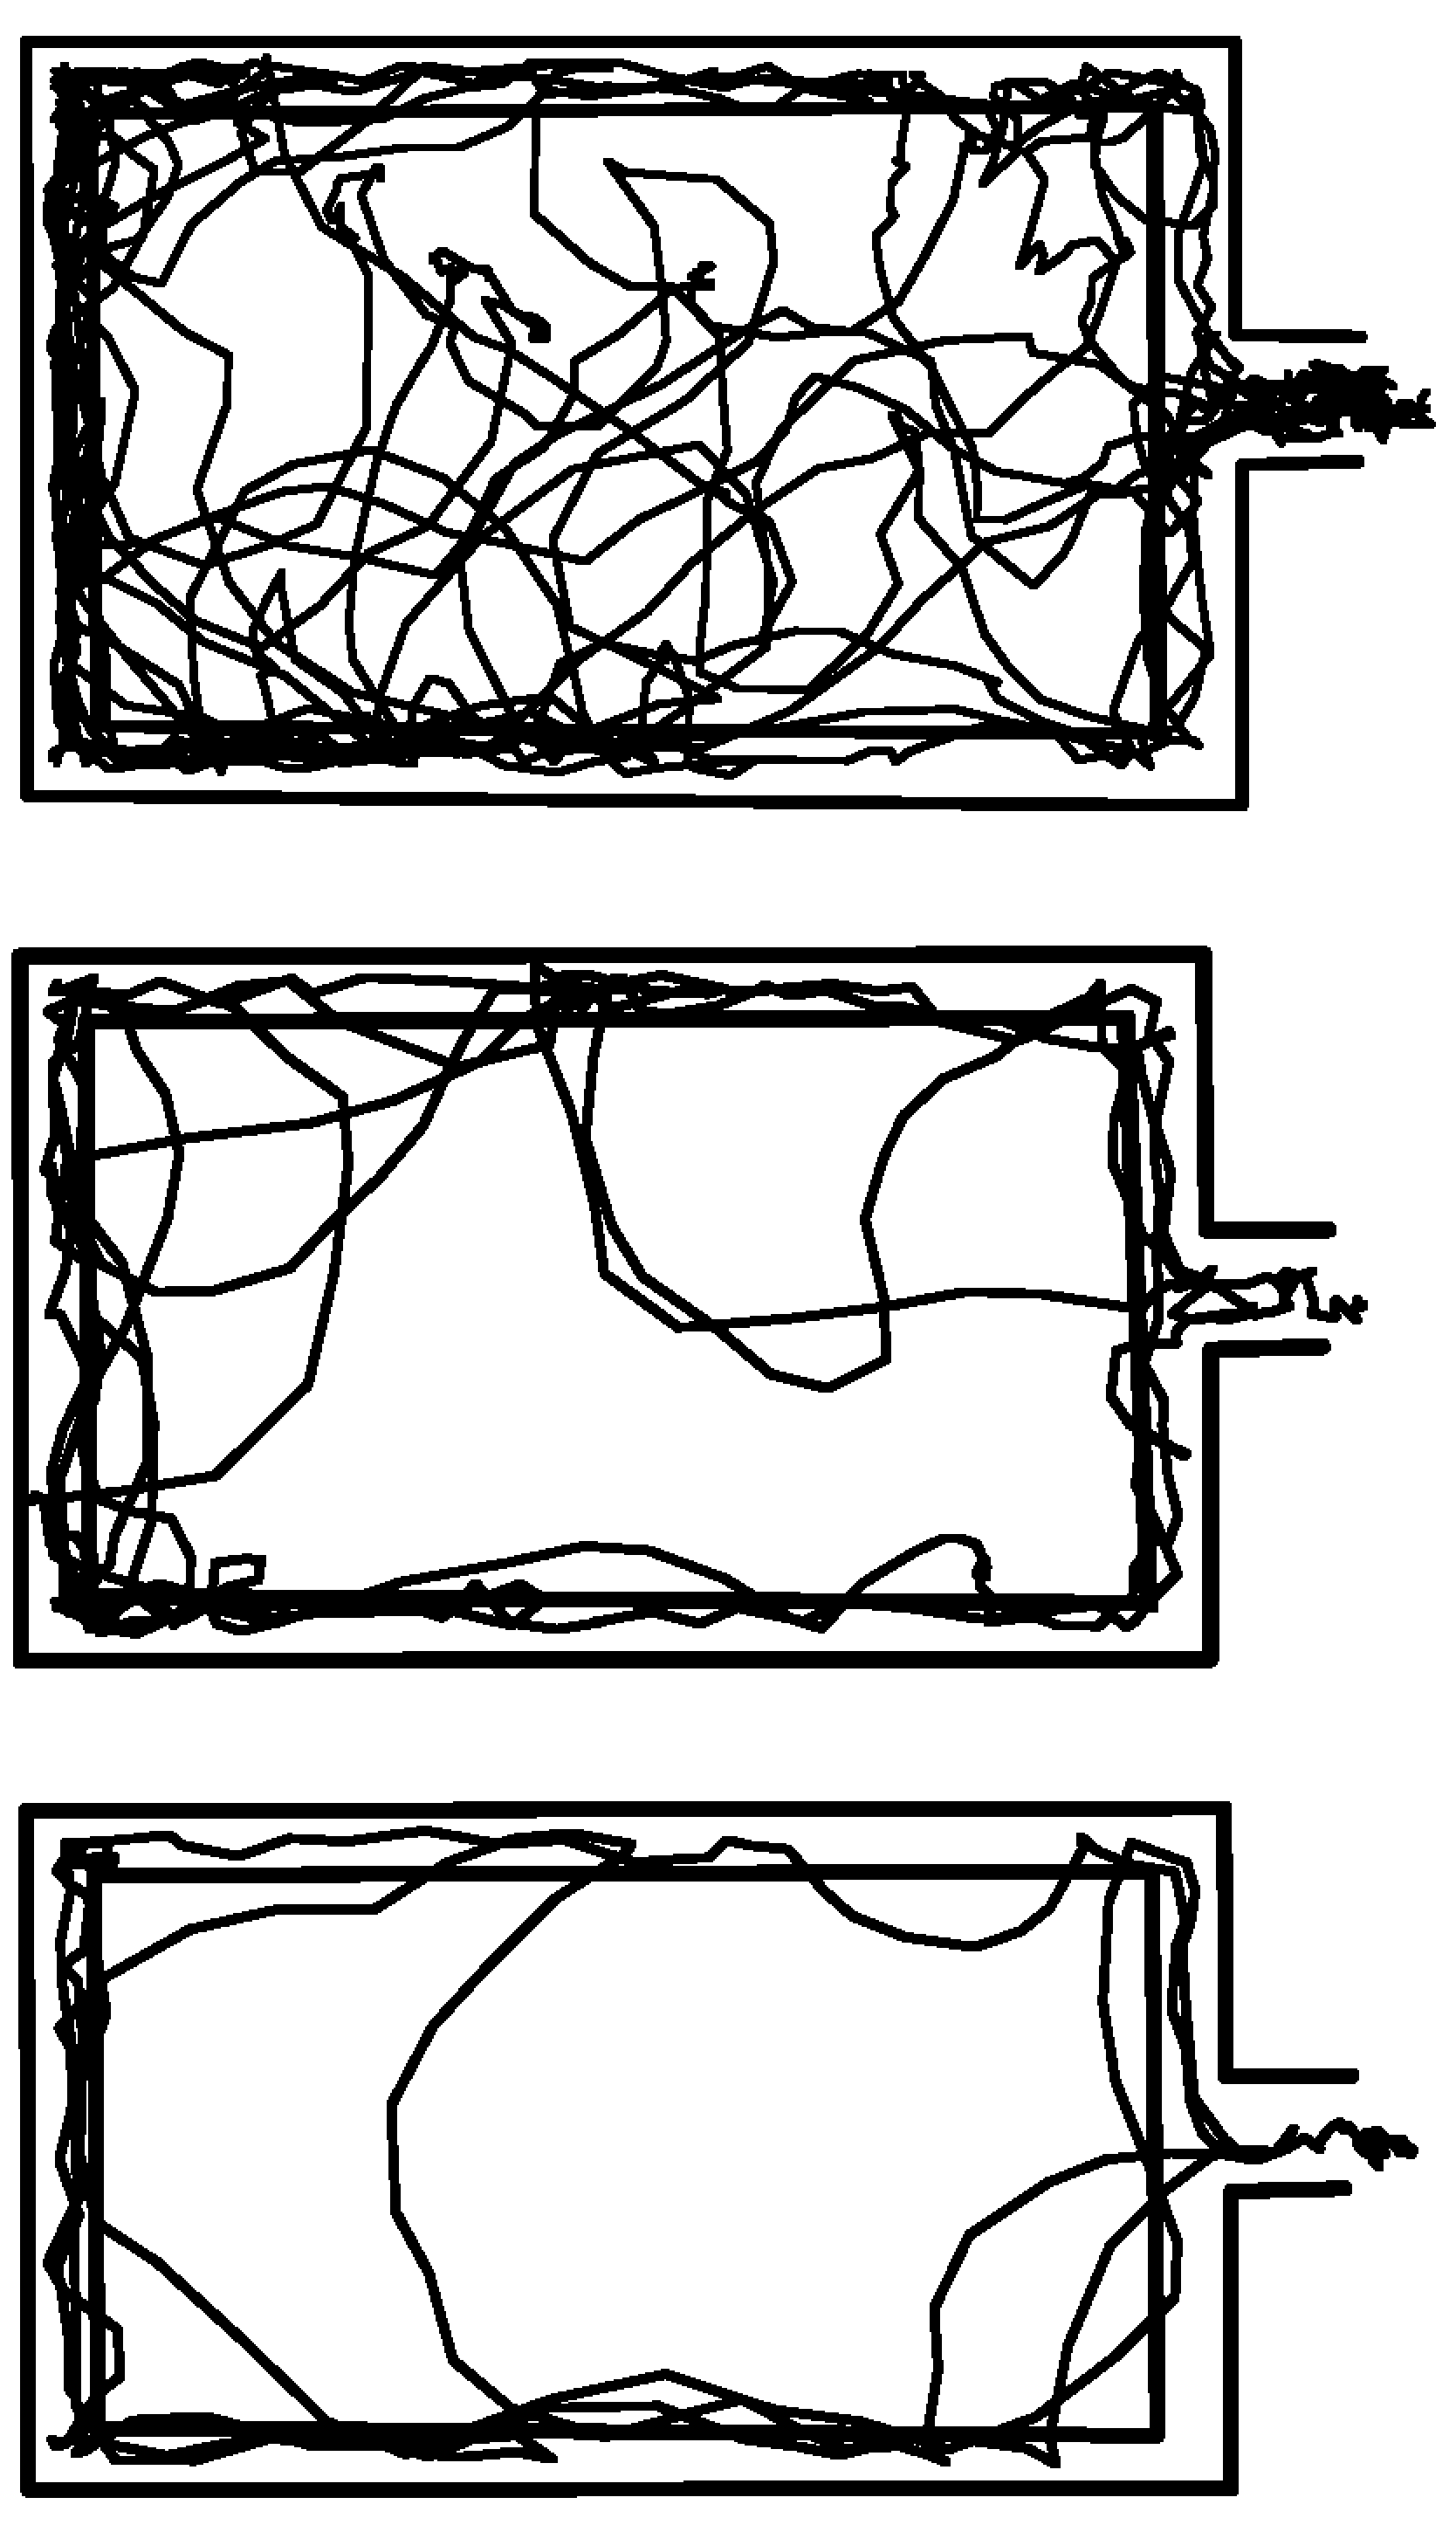
\includegraphics[width=0.65\linewidth]{10}
		\caption{\small\textit{\color{toanhocdoisong}Hình $7$. Từ trên xuống: Đường đi của kiến trinh sát khi khảo sát tổ được camera ghi lại trong lần khảo sát thứ nhất, thứ hai và thứ ba.}}
		\vspace*{-10pt}
	\end{figure}
	Theo các tác giả, số giao điểm của $L$ và $S$ được kiến trinh sát sử dụng để đánh giá diện tích của một vị trí làm tổ. Trong công thức ($4$), nếu ta thay các đường sợi tóc bằng một đường cong $L$ và rễ cây $R$ bằng đường cong $S$, công thức này vẫn đúng và diện tích có thể được xấp xỉ theo 
	\begin{align*}
		A = \frac{2SL}{\pi N}, \tag{$5$}
	\end{align*}
	với $N$ là số giao điểm của $S$ và $L$.
	\vskip 0.1cm
	Để kiểm chứng việc này, thí nghiệm được tiến hành với nhiều con kiến trinh sát khác nhau trên các loại hộp để làm tổ như trong hình vẽ.
	\vskip 0.1cm
	Trong thí nghiệm để chọn giữa hai tổ cùng chu vi (hình $8a$ và hình $8c$), kiến luôn chọn tổ có diện tích lớn hơn sau khi khảo sát cả hai. Do đó, diện tích chứ không phải chu vi mới là tiêu chí chọn tổ. Vì các tổ có một tấm chắn ở giữa (hình $8d$) cũng được chọn với khả năng tương tự như tổ bình thường, cho thấy số lần va chạm với chướng ngại vật trong tổ cũng không phải nhân tố quyết định.
	\begin{figure}[H]
		\vspace*{-5pt}
		\centering
		\captionsetup{labelformat= empty, justification=centering}
		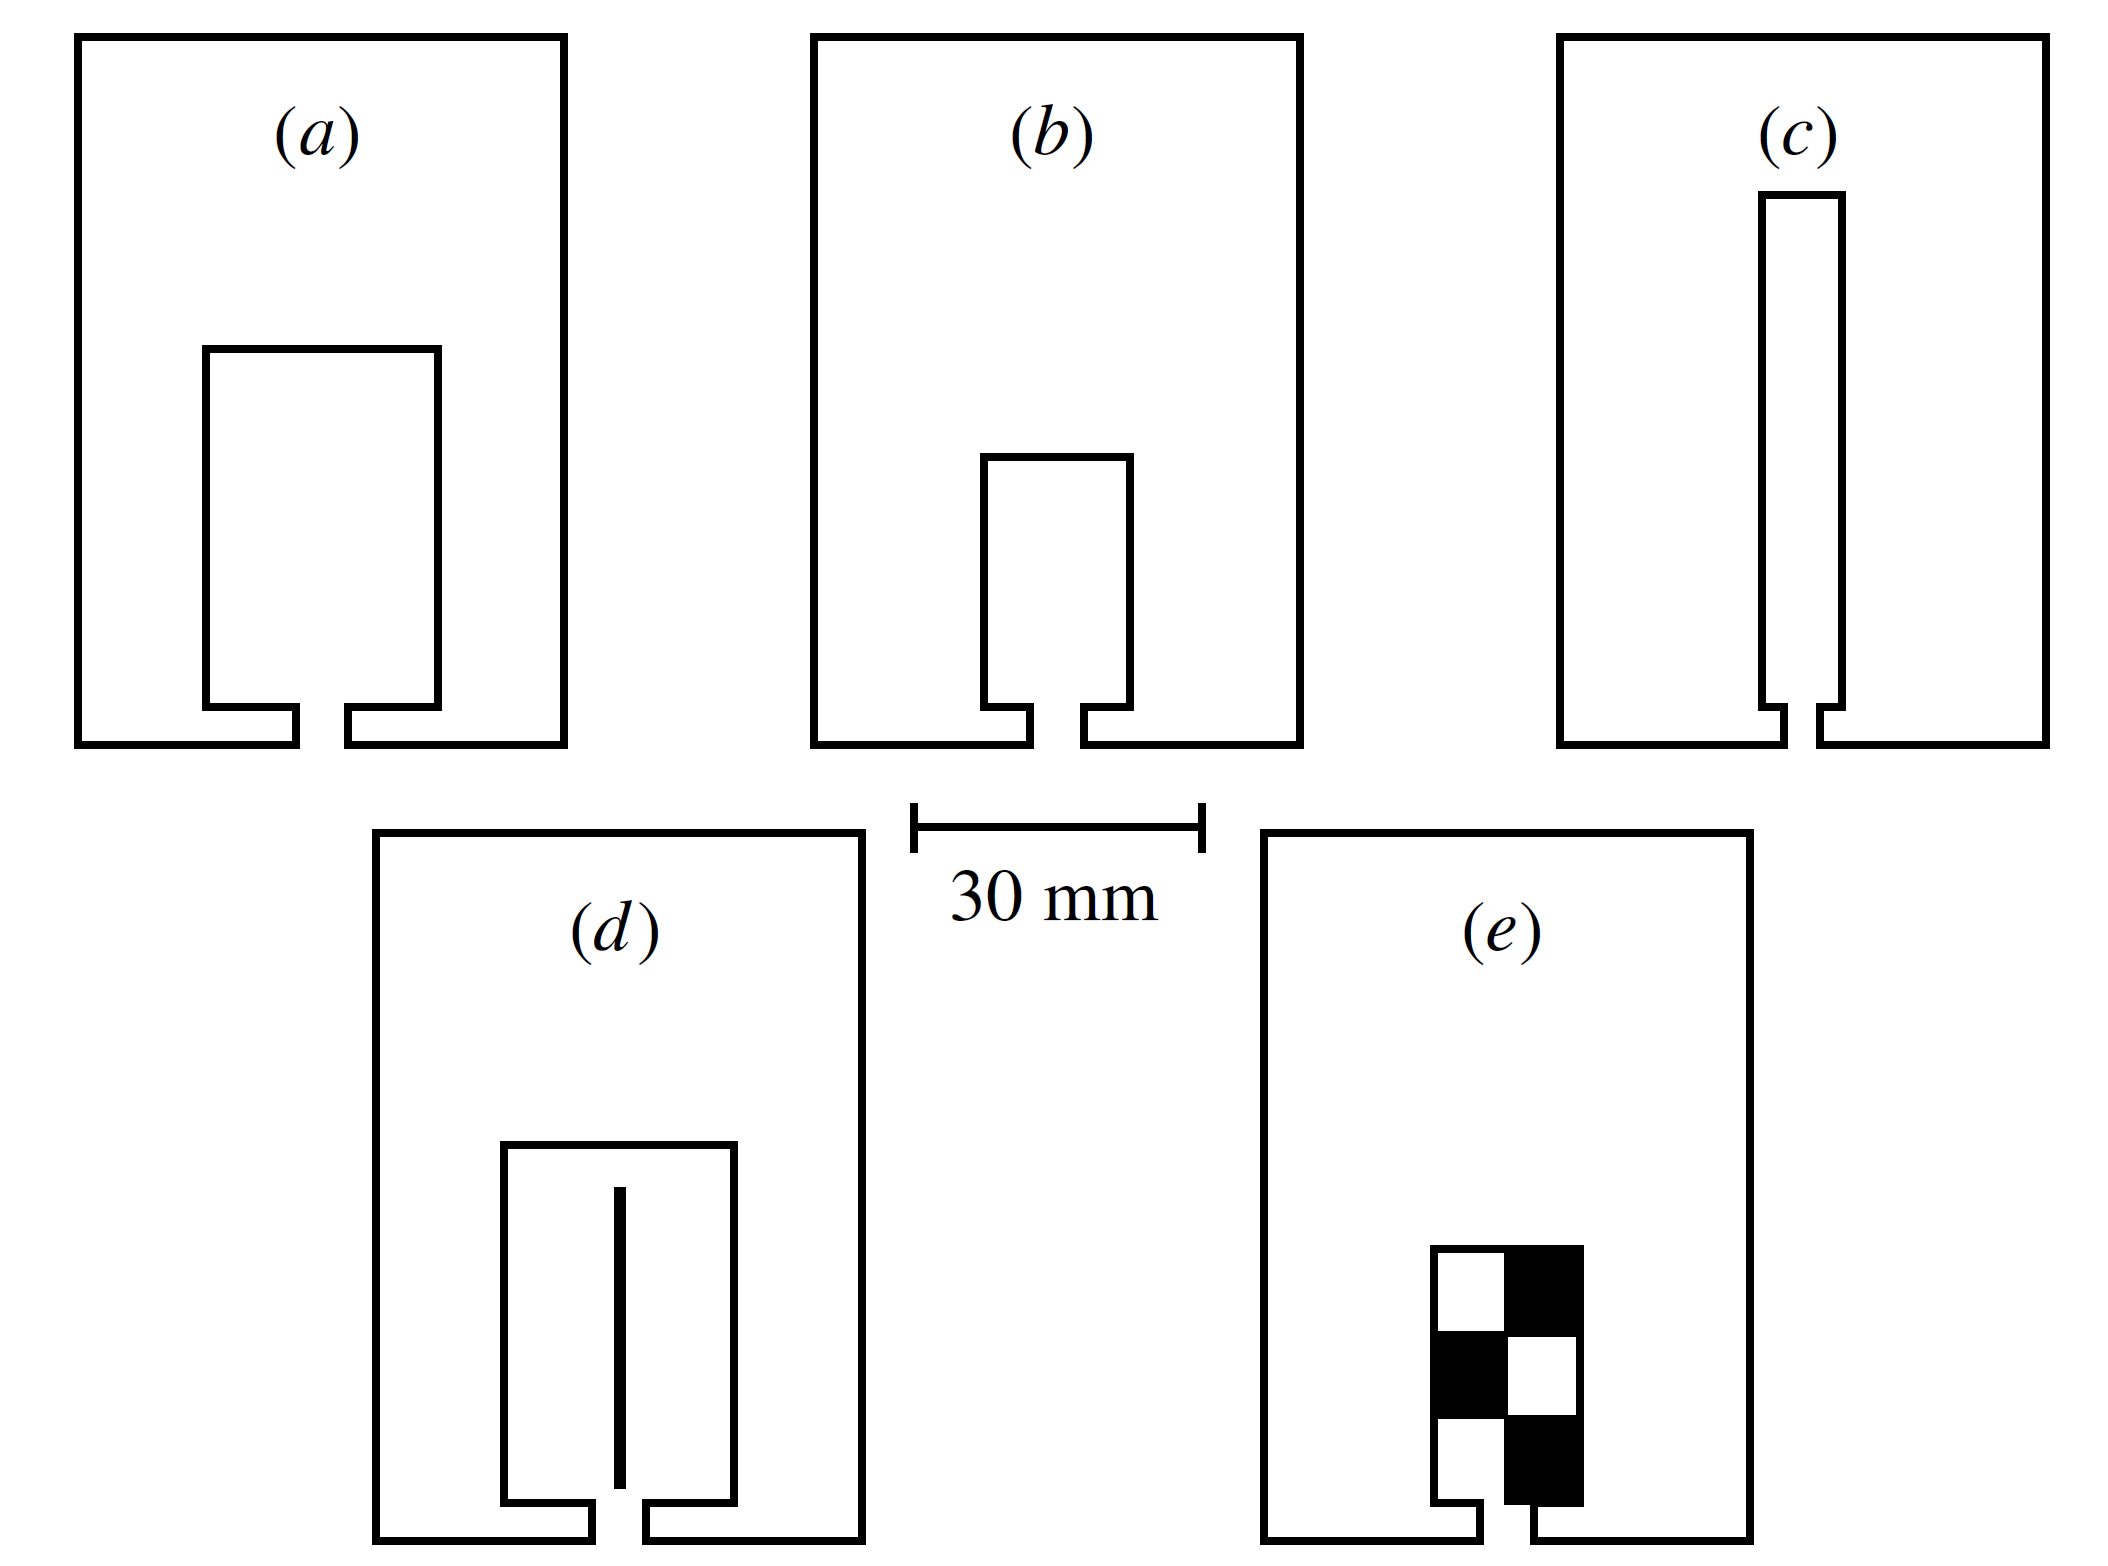
\includegraphics[width=1\linewidth]{11}
		\caption{\small\textit{\color{toanhocdoisong}Hình $8$. Các loại tổ được sử dụng trong thí nghiệm về việc chọn tổ của kiến trinh sát. $a)$ tổ tiêu chuẩn; $b)$ tổ đồng dạng và có diện tích bằng một nửa tổ tiêu chuẩn; $c)$ tổ có diện tích bằng một nửa tổ tiêu chuẩn nhưng có cùng chu vi; $d)$ tổ tiêu chuẩn có tấm chắn ở giữa; $e)$ tổ dạng $b$ với một nửa được phủ các tấm đệm có thể nhấc ra.}}
		\vspace*{-10pt}
	\end{figure}
	Thí nghiệm cũng cho thấy khi kiến trở lại lần thứ hai, nếu tổ đã được thay bằng một tổ mới hoặc một tổ đã được một con kiến khác đi qua, nó sẽ tiến hành khảo sát lại như là đang đi qua lần thứ nhất. Điều này cho thấy trong lần khảo sát thứ nhất, kiến sẽ lưu lại pheromone đánh dấu đường đi và pheromone này đặc trưng cho từng cá thể. Việc này cũng cho phép các con kiến không làm ảnh hưởng đến quá trình khảo sát của nhau khi một vị trí có thể được nhiều hơn một con kiến đến thăm dò.
	\vskip 0.1cm
	Nếu kiến trở lại lần thứ ba hoặc sau đó, thời gian nó tiến hành khảo sát cũng không khác nhiều lắm so với lần thứ hai, do đó có thể thấy pheromone chỉ được rải ở lần thăm dò thứ nhất còn các lần lặp lại sau để tăng độ chính xác của việc ước lượng.
	\vskip 0.1cm
	Loại tổ trong hình $8e$ được thiết kế đồng dạng với tổ trong hình $8a$ nhưng có diện tích bằng một nửa. Đồng thời, ở nền của loại tổ này, một nửa diện tích là các tấm đệm có thể lấy ra. Sau khi kiến khảo sát tổ dạng này lần thứ nhất, người ta sẽ lấy các tấm đệm ra trước khi kiến quay lại lần thứ hai. Khi kiến trở lại, do các vị trí có đệm bị lấy ra không còn pheromone nên số giao điểm của đường đi của nó trong lần thứ hai với đường đi trong lần thứ nhất sẽ giảm một nửa. Trong thí nghiệm chọn giữa tổ dạng $8a$ và dạng $8e$, một nửa số kiến chọn $8e$ dù diện tích chỉ có một nửa. Thí nghiệm với kích thước tổ lớn gấp đôi cho thấy khoảng cách $L$ của mỗi con kiến là không đổi giữa các tổ với diện tích khác nhau. Kết hợp với với ($5$), có thể thấy thấy kiến đánh giá diện tích theo tỉ lệ nghịch với tần số gặp giao điểm $\dfrac{N}{S}$.
	\vskip 0.1cm
	Việc nghiên cứu những thuật toán liên quan đến hành vi của kiến không chỉ có ý nghĩa về mặt sinh học mà còn có nhiều ứng dụng khác, ví dụ như trong việc lập trình điều khiển hành vi của robot.
	\vskip 0.1cm
	$\pmb{4.}$ \textbf{\color{toanhocdoisong}Lời kết}
	\vskip 0.1cm
	Lĩnh vực xác suất hình học còn có nhiều bài toán khác có giá trị về cả mặt lý thuyết lẫn thực tiễn. Pi cũng sẽ tiếp tục giới thiệu các bài toán này đến với độc giả trong tương lai không xa.
	\vskip 0.1cm
	\textbf{\color{toanhocdoisong}Tài liệu tham khảo}
	\vskip 0.1cm
	[$1$] Aigner, M., \& Ziegler, G. ($2004$). \textit{Proof from} THE BOOK. Springer--Verlag.
	\vskip 0.1cm
	[$2$] Mallon, E. B., \& Franks, N. R. ($2000$). Ants estimate area using Buffon's needle. \textit{Proc. R. Soc. Lond.} B($267$), $765-770$.
	\vskip 0.1cm
	[$3$] Mugford, S. T., Mallon, E. B., \& Franks, N. R. ($2001$). The accuracy of Buffon's needle: a rule of thumb used by ants to estimate area. \textit{Behavioral Ecology}, $12(6)$, $655-658$.
	\vskip 0.1cm
	[$4$] Newman, E. I. ($1966$). A Method of Estimating the Total Length of Root in a Sample. \textit{Journal of Applied Ecology}, $139-145$.
	\vskip 0.1cm
	[$5$] Ramaley, J. F. ($1969$). Buffon's Noodle Problem. \textit{The American Mathematical Monthly}, $78(8)$, $916-918$.
\end{multicols}